\section{Introduction}
\label{sec:Introduction}

\subsection{Overview} 
\paragraph{}
Ours is an increasingly visual culture and with the development of computing technology, people are no longer simply satisfied with just the visible but have a higher demand of visual effects.
% AR or image process
\par Augmented Reality (AR) is a strong and emerging presence in the IT market. Enhanced GPS systems are using AR to make it easier to get from point A to point B. The ability to augment a live view of displays in a museum with facts and figures is a natural use of the technology as well. With recent advances in computing power and technology, gaming applications with digital image processing are on the upswing, too. Head mounted systems are inexpensive and computing power is more portable than ever. 
\par Evidently, AR, an advanced technology, has furthered and enhanced several aspects of our life and the technology behind is really meaningful.

\subsection{Motivation}
\paragraph{}
In July 2016, an AR mobile game named Pokemon Go was released in certain countries, and in other regions over the next few months. The game uses the mobile devices GPS to locate, capture, battle, and train virtual creatures, called Pokemon, which are projected onto the camera in real-time to appear as if they are in the player's real-world location. 
\par
The game was referred to as a "social media phenomenon" which has brought people together from all walks of life. Over 231 million people engaged in 1.1 billion interactions that mentioned Pokemon Go on Facebook and Instagram in the month of July. Numerous media outlets referred to the surge in popularity as "Pokemon Go Mania", or simply "Pokemania". The massive popularity of the game resulted in several unusual positive effects. For example, the game enabled players to help catch criminals and to report crimes in progress, and has even aided law enforcement's community relations, albeit with caveats. Businesses also benefited from the nearby presence of PokeStops (or them being PokeStops themselves) with the concomitant influx of people, and the intense exploration of communities has brought local history to the forefront. The game was also seen bringing its players to places of worship, as many Pokegyms are located there. Despite some criticism by religious leaders, this was received positively by religious groups, who saw it as reminding adherents to come and pray.
\par
Pokemon Go was one of the most used and profitable mobile apps in 2016, having been downloaded more than 500 million times worldwide by the end of the year. It is credited with popularizing location-based and AR technology, promoting physical activity, and helping local businesses grow due to increased foot traffic. In May 2018, The Pokemon Company announced that the game had received over 800 million downloads worldwide, and it has 147 million monthly active users as of May 2018. As of September 2018, the game has grossed 2.01 billion dollars worldwide.

\subsection{The Gift Box Application}
\paragraph{}
This application seeks to explore the augmented-and-virtual-reality space by creating an Android app that allows users to attach virtual messages or objects at specific places in the real world. Virtual entities will be viewable and recoverable only by those individuals that the user selects. The locations of these objects are determined by a combination of GPS coordinates in conjunction with image processing keypointing.
\par Imagine a user with a mobile Android device. The user walks into a room and takes an image of a wall-hanging, as shown in Figure 1(a). The app allows the user to select a place in the image to which a virtual entity can be attached. This selection process can be partially automated. The user then selects a virtual object offered by the application or create one themselves. The virtual object will be later send to the recipient chosen by the user. Recipients are notified that a virtual gift has been granted to them and they are only given the location of that object. Each recipient must then navigate to the same room, scan the room with their app, and if they scan the targeted room region, they will receive the virtual gift. A mock-up of the gifting process is shown in Figure 1(b).

\begin{figure}[H]
\centering
\begin{minipage}[t]{0.5\textwidth}
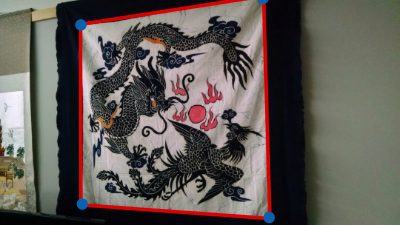
\includegraphics[width=.95\textwidth]{section01/assets/giftbox_1.png}
\subcaption{}
\end{minipage}%
\begin{minipage}[t]{0.5\textwidth}
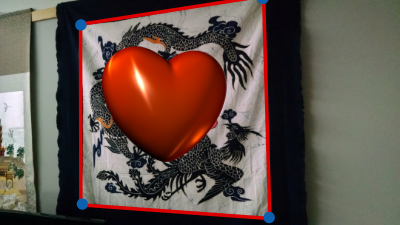
\includegraphics[width=.95\textwidth]{section01/assets/giftbox_2.png}
\subcaption{}
\end{minipage}%

\caption[Short Caption]{Example Result}
\end{figure}

\paragraph{} This application also contains a web interface that allows user to have a general idea of the whole project before they download the android application. Users can not only view and edit their profile but also manage their friends list online. If you don't have your Android device with you it will be a good choice to check if you have any recently received gifts online as well. At the same time, it leaves an interface for administrator users to add more virtual gifts into the database and manage user activities.



